
\documentclass[a4paper, 12p]{paper} 
\usepackage[margin=2.5cm]{geometry}
\usepackage{amsmath}
\usepackage{graphicx}
\usepackage{lipsum}
\usepackage{xcolor}
\usepackage{booktabs}
\usepackage{float}
\usepackage{subfigure}
\usepackage{titling}
\usepackage{kotex}
\usepackage{gensymb}
\usepackage{minted}

\def\code#1{\texttt{#1}}
\sectionfont{\large\sf\bfseries\color{black!70!blue}}
\date{\vspace{-5ex}}
\renewcommand{\familydefault}{\sfdefault}
\renewcommand{\baselinestretch}{1.3} 

\pretitle{\centering\LARGE\bfseries}
\posttitle{\par}
\preauthor{\begin{flushright}\large}
\postauthor{\end{flushright}}

\title{Spatial Filtering of Gray Images}
\author{전자공학과 20161453 김규래}

\begin{document} 
\maketitle\hrule{}\bigskip

\section{Overview}
이번 과제의 목적은 spatial filtering 을 구현해보고, padding 을 적용한 다음 각각의 특성을 특성을 이해하는 것이다. 또한 Gaussian smoothing, box smoothing, sobel edge detection, laplacian edge enhancement 와 같은 광범위하게 사용되는 필터들을 사용해봄으로서 이들의 특성 또한 파악하는 것이 목표이다. 

구현한 함수들은 다음과 같으며, 순서대로 spatial filtering 함수, gaussian kernel 생성 함수, laplacian kernel 생성 함수, sobel kernl 생성 함수, box kernel 생성 함수이다.

  \begin{minted}
    [frame=lines,
      framesep=2mm,
      baselinestretch=0.5]{cpp}
inline cv::Mat conv2d(cv::Mat const& src, kernel_t const& kernel, pad_type pad);

inline kernel_t kernel::gaussian_filter(float sigma, size_t n);

inline kernel_t kernel::laplacian_filter(bool is_4_direction)

inline kernel_t kernel::sobel_filter(bool is_x_direction)

inline kernel_t kernel::box_filter(size_t n)
  \end{minted}

 \subsection{padding}
 conv2d 는 기본적으로 'same' 모드로, 입력되는 \code{src} 영상과 동일한 크기의 영상을 반환한다. Finite discrete domain 에서는 spatial filtering 을 수행할 경우 정보의 손실이 발생하면서 영상의 크기가 줄어들기 때문에 같은 크기를 유지하기 위해서는 보정을 해야한다. 이 보정을 padding 이라고 하며, 일반적으로는 다음과 같은 3가지를 사용한다

 \begin{enumerate}
   \item \textbf{Zero padding} 영상의 바깥을 전부 0 으로 취급.
   \item \textbf{Extension padding} 영상의 바깥부분의 픽셀들을 영상에서 가장 가까운 픽셀로 대체.
   \item \textbf{Mirror padding} 영상의 바깥 부분에 영상을 대칭으로 연장.
 \end{enumerate}

 Zero padding 의 경우에는 접근 인덱스가 영상의 테두리를 벗어나는 경우 영상의 값을 0 으로 대체하면 되고, extension padding 의 경우 접근 인덱스를 clamping 해서 구현할 수 있다. 마지막으로 mirror padding 은 인덱스가 영상을 벗어나는 만큼 영상의 방향으로 인덱스를 변환하는 것으로 구현할 수 있다. 본 구현에서는 zero padding 과 extension padding 을 구현하였으며 \code{conv2d} 함수에 인자를 전달해서 선택을 할 수 있게 하였다.

\section{Implementation}
언어는 C++14 를 사용하였으며 빌드 시스템은 CMake 로 구성하였다. 리눅스 환경에 맞게 작성이 됐기 때문에 리눅스에서 빌드할 것을 권장한다.

\subsection{External Dependencies}
외부 라이브러리로는 OpenCV\footnote{https://opencv.org/} 를 사용하였다. OpenCV 에서는 다양한 영상처리 관련 루틴들을 제공하고 있으나, 본 과제에서는 \code{cv::imshow()} 와 \code{cv::imread()}, \code{cv::imwrite()} 와 같은 입출력 관련 함수들만 사용하였다.

\subsection{Installation}
시스템에 OpenCV 가 표준 경로에 설치돼있을 경우 CMake 에서 자동으로 인식을 할 것이다. 별도의 경로에 설치돼 있을 경우 \code{OpenCV\_ROOT\_DIR} 변수를 CMake 에 플래그로 넘김으로써 경로를 알려줄 수 있다. Blaze 의 경우에는 함께 첨부돼 있기 때문에 별도의 작업이 필요하지 않다. 다음과 같이 입력하면 빌드를 할 수 있다. 

\begin{align*}
  & \code{mkdir build \&\& cd build} \\
  & \code{cmake -G ``Unix Makefiles'' ..} \\
  & \code{make}
\end{align*}

\subsection{구현1}
구현1 에서는 box kernel 과 gaussian kernel 을 이용하여 smooting 연산을 수행하는 것이 목표이다. Gaussian kernel 의 경우에는 Eq.\ref{eq:gauss} 를 이용하여 생성하였다. 이 때 $k$ 는 normalization constant 로, 생성되는 커널의 모든 coefficient 들의 합의 역수이다. Eq.\ref{eq:gauss_kern} 는 $\sigma = 1.0, n = 7$ 일 때 생성되는 gaussian blur 커널이다.

\begin{equation}
  K_{\text{gauss}}(x, y, \sigma) = \frac{1}{k} \exp(-\frac{x^2 + y^2}{2 \sigma^2})\label{eq:gauss}
\end{equation}

\begin{equation}
  K_{\text{gauss}} =
  \begin{pmatrix}
     0.000036 & 0.000363 & 0.001446 & 0.002291 & 0.001446 & 0.000363 & 0.000036 \\
     0.000363 & 0.003676 & 0.014662 & 0.023226 & 0.014662 & 0.003676 & 0.000363 \\
     0.001446 & 0.014662 & 0.058488 & 0.092651 & 0.058488 & 0.014662 & 0.001446 \\
     0.002291 & 0.023226 & 0.092651 & 0.146768 & 0.092651 & 0.023226 & 0.002291 \\
     0.001446 & 0.014662 & 0.058488 & 0.092651 & 0.058488 & 0.014662 & 0.001446 \\
     0.000363 & 0.003676 & 0.014662 & 0.023226 & 0.014662 & 0.003676 & 0.000363 \\
     0.000036 & 0.000363 & 0.001446 & 0.002291 & 0.001446 & 0.000363 & 0.000036 \\
  \end{pmatrix}\label{eq:gauss_kern}
\end{equation}

Box kernel 은 Eq.\ref{eq:box} 와 같이 생성하였으며 이를 통해서 $n=3$ 일 때 생성되는 커널은 Eq.\ref{eq:box_kern} 와 같다. 이 때 $n$ 은 box kernel 의 가로, 세로 크기이다.

\begin{equation}
  K_{\text{box}}(x, y, n) = \frac{1}{n^2}\label{eq:box}
\end{equation}
\begin{equation}
  K_{\text{gauss}} =
  \begin{pmatrix}
     1/9 & 1/9 & 1/9 \\
     1/9 & 1/9 & 1/9 \\
     1/9 & 1/9 & 1/9
  \end{pmatrix}\label{eq:box_kern}
\end{equation}

다음은 제시된 영상 \code{Test\_pattern.tif} 에 gaussian smoothing 을 적용했을 때의 결과이다.

\begin{figure}[H]
\centering
\subfigure[n=7, $\sigma$=1, extension padding]{
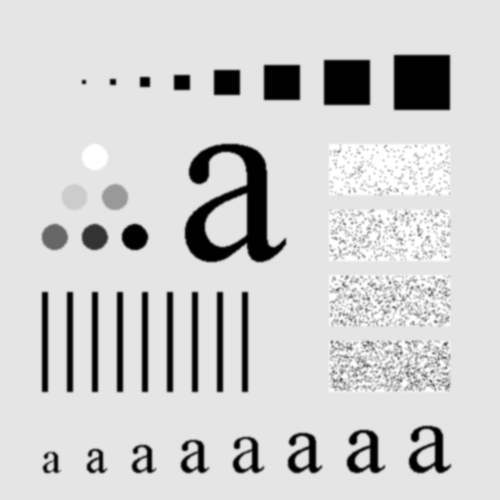
\includegraphics[scale=0.22]{../data/gaussian1_extpad.png}
}
\subfigure[n=21, $\sigma$=3.5, extension padding]{
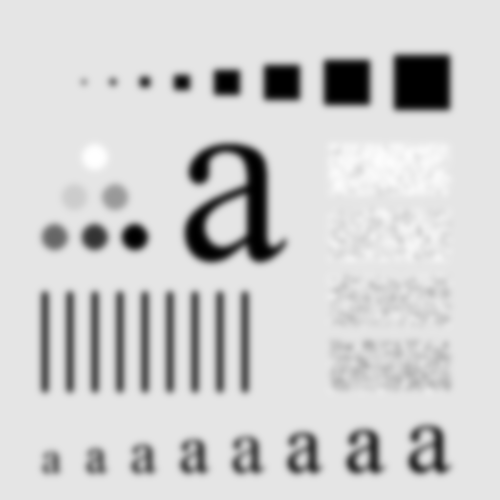
\includegraphics[scale=0.22]{../data/gaussian2_extpad.png}
}
\subfigure[n=43, $\sigma$=7, extension padding]{
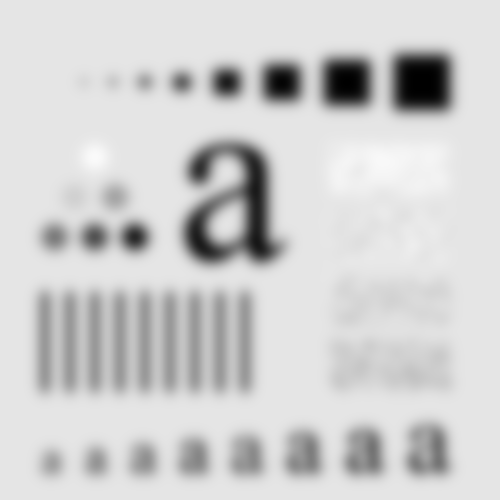
\includegraphics[scale=0.22]{../data/gaussian3_extpad.png}
}
\subfigure[n=7, $\sigma$=1, zero padding]{
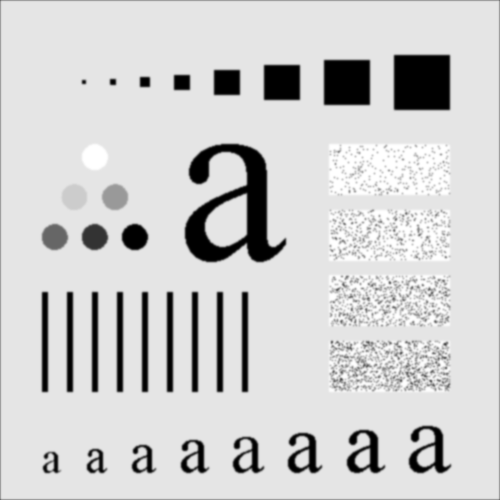
\includegraphics[scale=0.22]{../data/gaussian1_zeropad.png}
}
\subfigure[n=21, $\sigma$=3.5, zero padding]{
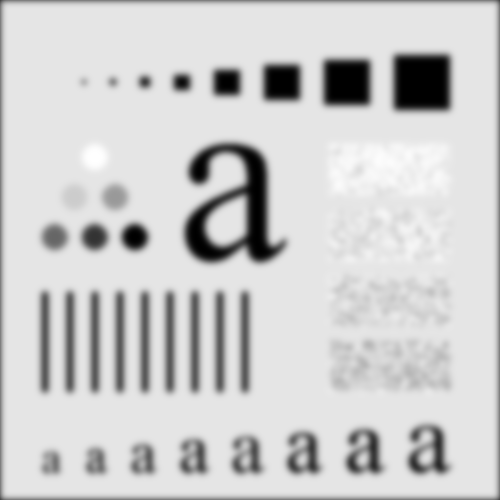
\includegraphics[scale=0.22]{../data/gaussian2_zeropad.png}
}
\subfigure[n=43, $\sigma$=7, zero padding]{
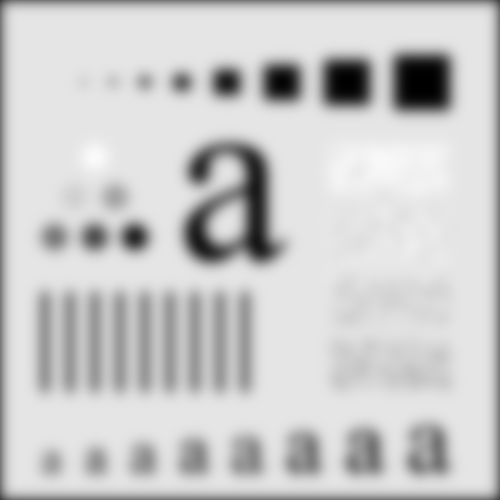
\includegraphics[scale=0.22]{../data/gaussian3_zeropad.png}
}
\caption{Gaussian filtering 을 적용했을 때의 모습. (열) kernel size 와 $\sigma$ 의 값에 따른 차이. (행) extension padding 과 zero padding 여부에 따른 차이}\label{fig:gauss_result}
\end{figure}

Fig.\ref{fig:gauss_result} 를 보면 gaussian filtering 을 적용했을 때의 효과를 볼 수 있다. Kernel 의 사이즈, $\sigma$ 가 증가함에 따라 영상의 선명도가 확연히 감소하는 것을 확인할 수 있다. 또한 zero padding 을 사용할 경우 영상의 테두리 부분에 검은색으로 왜곡이 발생하는 것을 볼 수 있다.

\begin{figure}[H]
\centering
\subfigure[n=3, extension padding]{
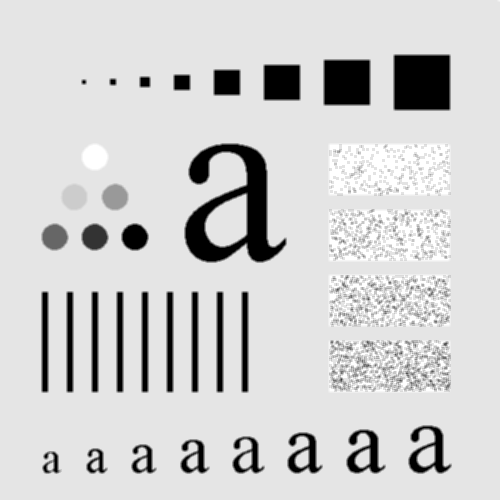
\includegraphics[scale=0.22]{../data/box1_extpad.png}
}
\subfigure[n=13, extension padding]{
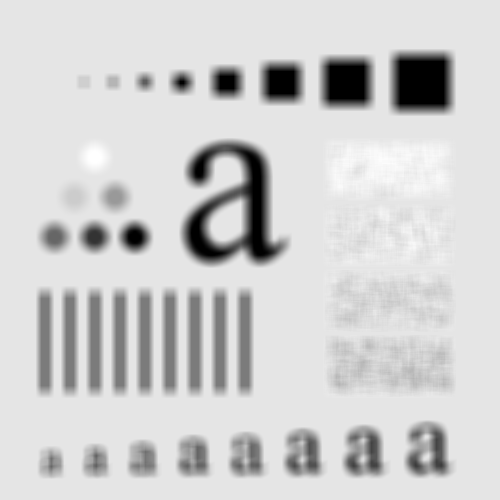
\includegraphics[scale=0.22]{../data/box2_extpad.png}
}
\subfigure[n=25, extension padding]{
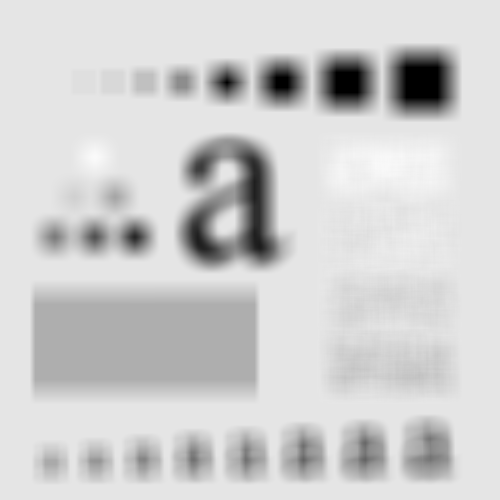
\includegraphics[scale=0.22]{../data/box3_extpad.png}
}
\subfigure[n=3, zero padding]{
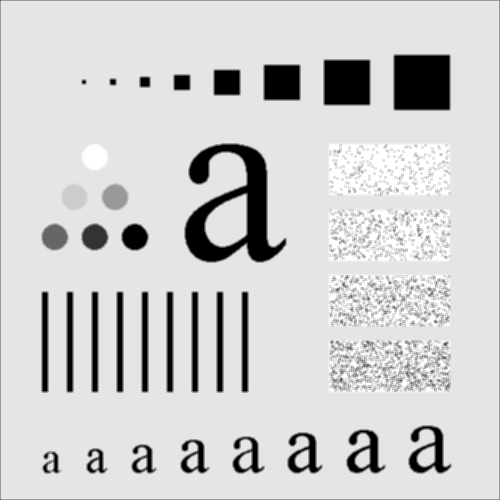
\includegraphics[scale=0.22]{../data/box1_zeropad.png}
}
\subfigure[n=13, zero padding]{
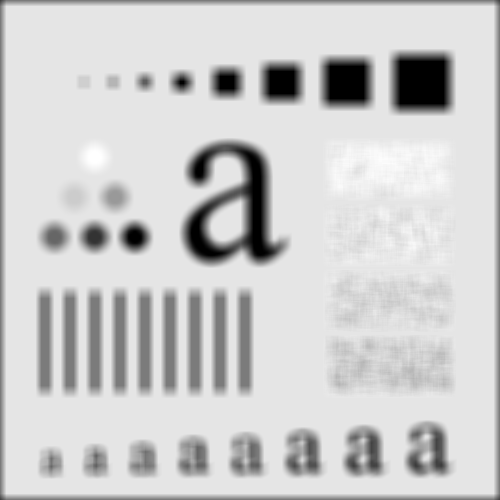
\includegraphics[scale=0.22]{../data/box2_zeropad.png}
}
\subfigure[n=25, zero padding]{
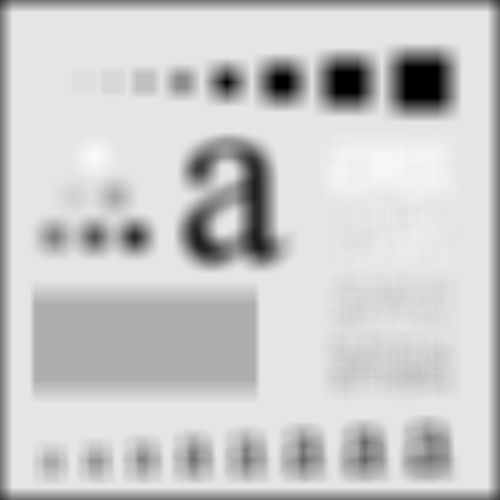
\includegraphics[scale=0.22]{../data/box3_zeropad.png}
}
\caption{Box filtering 을 적용했을 때의 모습. (열) kernel size 와 $\sigma$ 의 값에 따른 차이. (행) extension padding 과 zero padding 여부에 따른 차이}\label{fig:box_result}
\end{figure}

Box filtering 을 사용할 때의 결과는 Fig.\ref{fig:box_result} 에서 볼 수 있다. 전체적으로는 gaussian filtering 과 비슷하게 영상의 선명도 떨어지는 효과를 얻는 것을 볼 수 있다. Kernel 의 크기가 증가할수록 선명도가 감소한다. 또한 gaussian filtering 에서와 비슷하게 zero padding 을 사용하는 경우에 태두리에 검은색 왜곡이 발생한다.

\textbf{검토사항} Box kernel 은 x축과 y축에 대해서 moving average filter 와 유사한 형태를 띈다. Moving average filter는 high frequency 신호의 강도가 약해지는 low pass filter 이기 때문에, 주어진 영상의 수직선과 같이 x축을 따라서 변화가 크게 발생하는(주파수가 큰) 신호의 경우 필터링돼 버린다. 그 효과로 수직선들 사이의 경계가 흐려진 것을 시각적으로 확인할 수 있다. Spatial domain 에서 생각을 할 경우 box kernel 효과는 kernel 의 크기만큼의 픽셀들을 평균 내버리는 것이기 때문에, 수직선의 경계가 뭉개져 버린 것으로 생각을 할 수 있다.

\subsection{구현2}
구현2 에서는 laplacian kernel 을 구현해서 edge enhancement, image sharpening 효과를 확인하는 것이 목적이다. 사용하는 kernel 은 2가지 종류이며, 각각 4-direction laplacian kernel~\ref{eq:4_laplace_kern} 과 8-direction laplacian kernel~\ref{eq:8_laplace_kern} 이다. 이 필터의 경우 제시된 \code{Boy.tif} 영상을 이용하였다.

\begin{equation}
  K_{\text{laplace-4}} =
  \begin{pmatrix}
     0  & -1 & 0 \\
     -1 &  4 & -1 \\
     0  & -1 & 0 
  \end{pmatrix}\label{eq:4_laplace_kern}
\end{equation}

\begin{equation}
  K_{\text{laplace-8}} =
  \begin{pmatrix}
     -1  & -1 & -1 \\
     -1  &  8 & -1 \\
     -1  & -1 & -1 
  \end{pmatrix}\label{eq:8_laplace_kern}
\end{equation}


Fig.~\ref{fig:laplace_result} 를 보면 laplacian filter 를 이용해서 추출한 edge response 를 볼 수 있다.
\begin{figure}[hbtp]
\centering
\subfigure[4 direction, zero padding]{
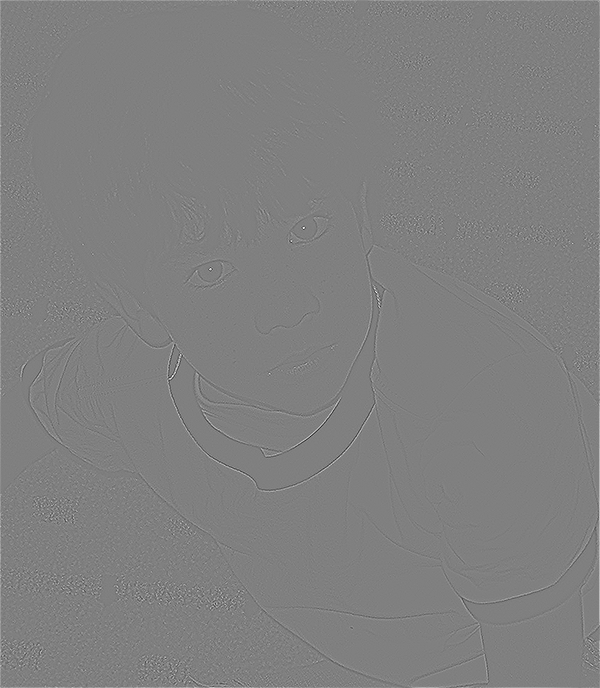
\includegraphics[scale=0.24]{../data/laplace4_zeropad.png}
}
\subfigure[8 direction, zero padding]{
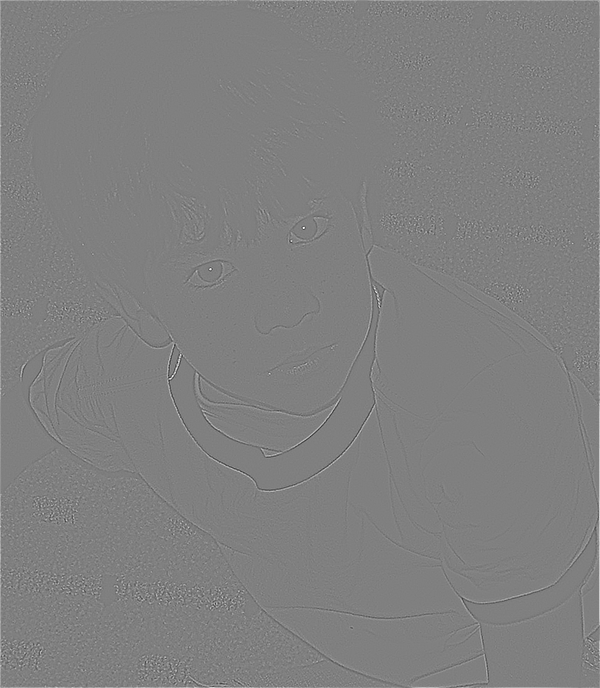
\includegraphics[scale=0.24]{../data/laplace8_zeropad.png}
}
\subfigure[4 direction, extension padding]{
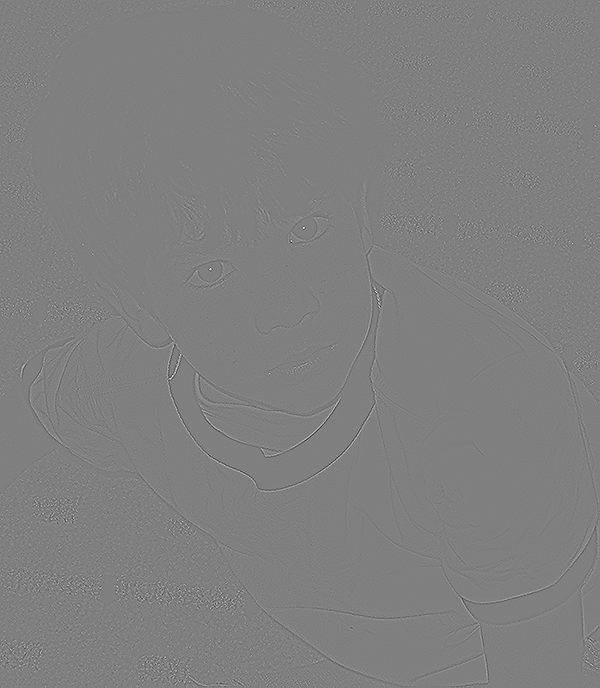
\includegraphics[scale=0.24]{../data/laplace4_extpad.png}
}
\subfigure[8 direction, extension padding]{
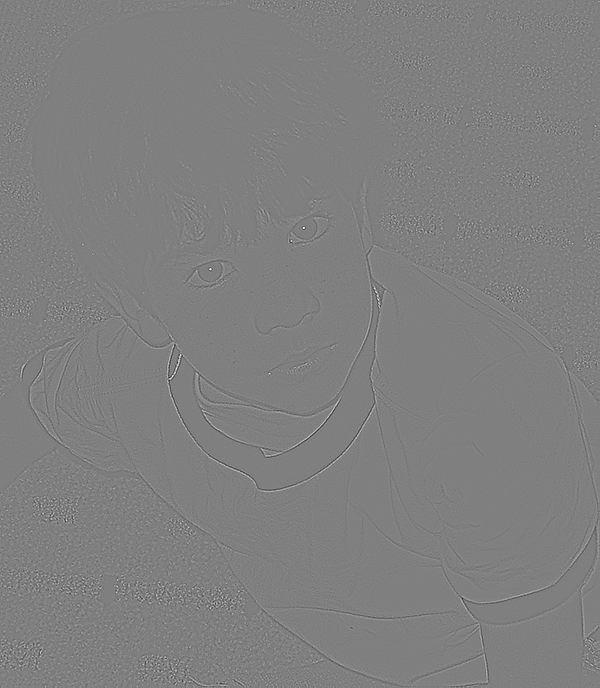
\includegraphics[scale=0.24]{../data/laplace8_extpad.png}
}
\caption{Laplacian filter을 적용한 값. (열) direction 에 따른 차이. (행) extension padding 과 zero padding 여부에 따른 차이}\label{fig:laplace_result}
\end{figure}

시각적으로 볼 때는 4-direction 과 8-direction 의 추출효과는 큰 차이가 없다. 다만 이는~Fig.~\ref{fig:laplace_result}의 영상들이 normalization 과 8-bit quantization 을 거쳤다는 점을 고려해야 한다. Normalization 과 quantization 을 거치지 않았을 때는 magnitude 가 차이를 보였을 가능성이 있다. 여기서 눈여겨볼 수 있는 점은 이전 Section 의 smoothing filter 들과 다르게 zero padding 과 extension padding 이 큰 차이를 보이지 않는다는 점이다. 이는 사용되는 kernel 의 사이즈가 크지 않고, 사용된 영상의 테두리 근처가 어두운 색이라서 edge 특성이 강하지 않기 때문으로 보인다. 아래는 원본 영상과 laplacian kernel 로 추출한 edge response 를 더했을 때의 결과물이다.

\begin{figure}[hbtp]
\centering
\subfigure[원본영상]{
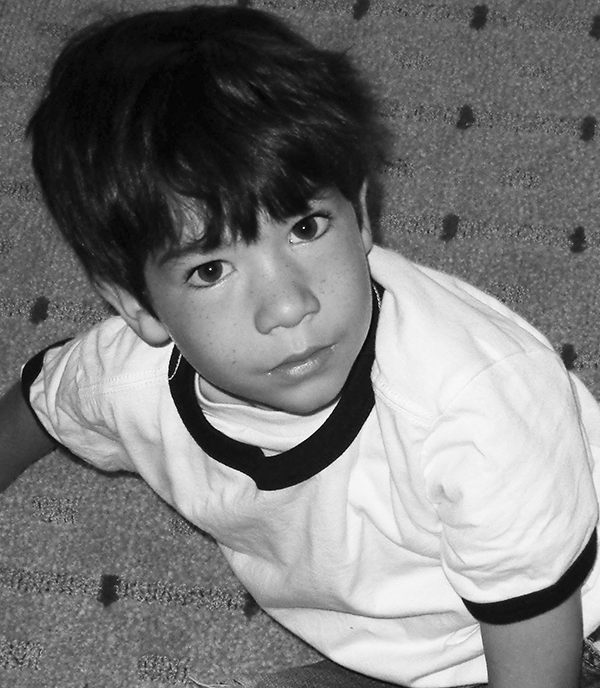
\includegraphics[scale=0.21]{../data/Boy.png}
}
\subfigure[4 direction]{
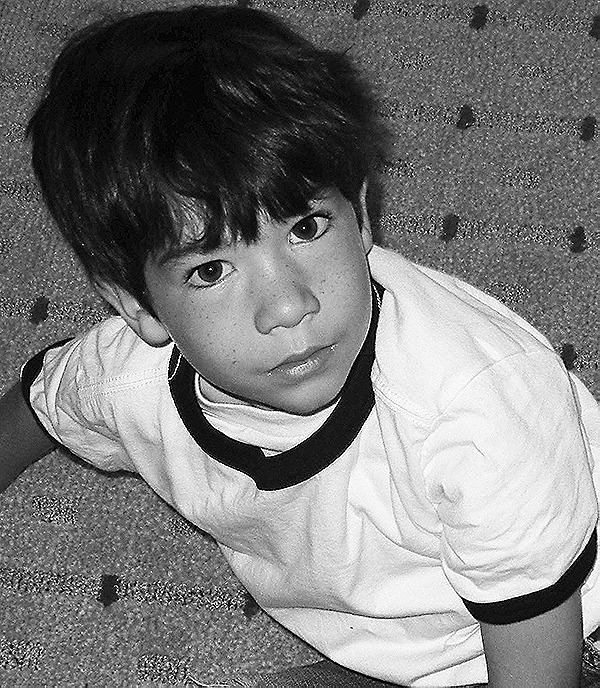
\includegraphics[scale=0.21]{../data/laplace4_en_extpad.png}
}
\subfigure[8 direction]{
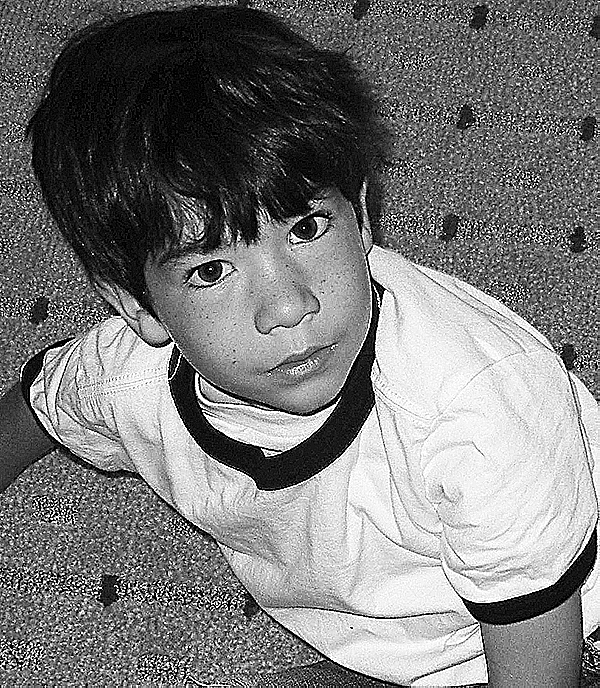
\includegraphics[scale=0.21]{../data/laplace8_en_extpad.png}
}
\caption{Laplacian filter 를 이용한 edge enhancement 적용 효과}\label{fig:edgeenhance_result}
\end{figure}

Fig.~\ref{fig:edgeenhance_result} 에서 edge enhancement 효과를 확인할 수 있다. Zero padding 과 extension padding 이 큰 차이를 보이지 않는 만큼, 여백이 부족하여 zero padding 을 적용한 영상은 제시하지 않았다. 다만 제출한 소스코드에서는 zero padding 을 적용한 영상 또한 생성을 한다.

결과를 보면 원본 영상에 비해 edge enhancement 를 적용한 영상들이 더 선명하다는 것을 시각적으로 확인할 수 있다. 또한 8-direction laplacian kernel 을 사용했을 때가 4-direction kernel 을 사용했을 때보다 선명도가 높은 것으로 나타난다. 이를 통해서 단순히 추출된 edge response 영상에서는 확인하기 힘든 두 kernel 간의 magnitude 차이가 존재함을 추론할 수 있다.

\subsection{구현3}
마지막으로 구현3 에서는 sobel kernel 을 사용하여 edge detection 을 수행하였다. 사용한 kernel 은~\ref{eq:sobelx_kern}, \ref{eq:sobely_kern} 로 각각 x축과 y축 방향으로 central differentiation 을 수행한다.

\begin{equation}
  K_{\text{sobel}_x} =
  \begin{pmatrix}
     -1  & 0 & 1 \\
     -2  & 0 & 2 \\
     -1  & 0 & 1 
  \end{pmatrix}\label{eq:sobelx_kern}
\end{equation}

\begin{equation}
  K_{\text{sobel}_y} =
  \begin{pmatrix}
     -1  & -2 & -1 \\
      0  &  0 &  0 \\
      1  &  2 &  2 
  \end{pmatrix}\label{eq:sobely_kern}
\end{equation}

\begin{figure}[hbtp]
\centering
\subfigure[$x$-axis direction, zero padding]{
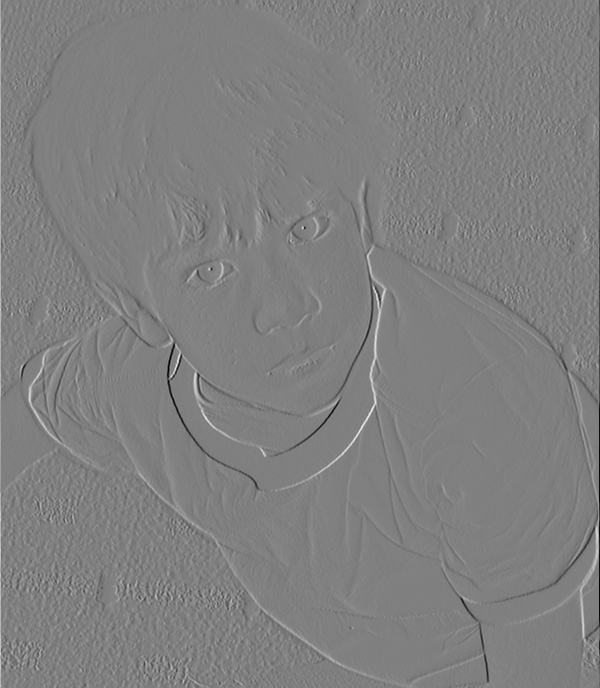
\includegraphics[scale=0.24]{../data/sobelx_zeropad.png}
}
\subfigure[$y$-axis direction, zero padding]{
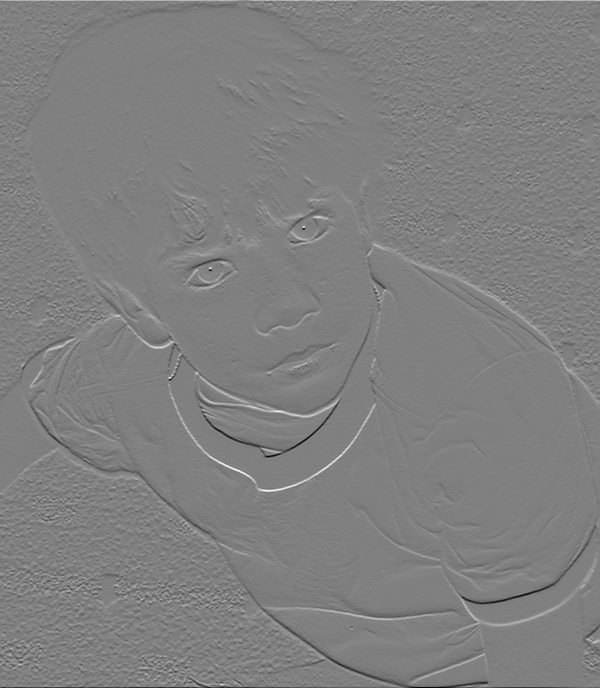
\includegraphics[scale=0.24]{../data/sobely_zeropad.png}
}
\subfigure[$x$-axis direction, extension padding]{
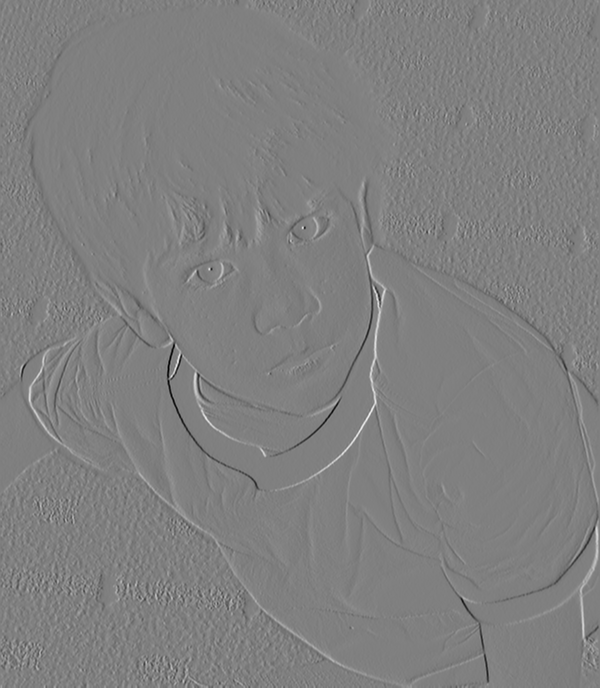
\includegraphics[scale=0.24]{../data/sobelx_extpad.png}
}
\subfigure[$y$-axis direction, extension padding]{
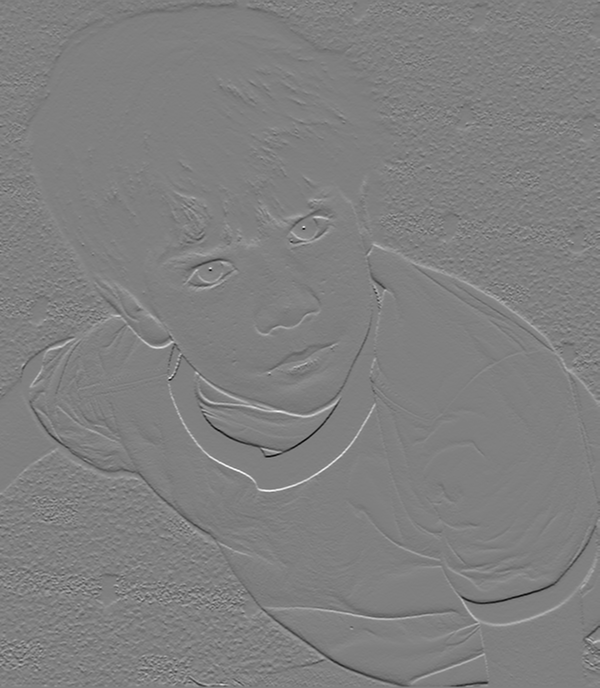
\includegraphics[scale=0.24]{../data/sobely_extpad.png}
}
\caption{Sobel operator를 적용한 값. (열) direction 에 따른 차이. (행) extension padding 과 zero padding 여부에 따른 차이}\label{fig:sobel_result}
\end{figure}

Sobel operator 를 적용했을 때의 결과는 Fig.~\ref{fig:sobel_result} 에서 볼 수 있다. $x$-axis 로 sobel operator 를 적용했을 때는 세로로 filter response 가 크게 나타나고, $y$-axis 로 적용했을 때는 가로로 filter response 가 크게 나타난 것을 볼 수 있다. 또한 기준으로 한 방향에 따라서 비슷한 형태의 엣지라도 특정 영역에서는 response 가 양수로 나타났는데 반해 특정 영역에서는 음수로 나타난 것을 알 수 있다. 따라서 의미 있는 값을 얻어내기 위해서는 별도로 Norm 연산을 취해야 하나, 본 과제에서는 요구되지 않았으므로 생략 하였다. 마지막으로, laplacian filter 를 적용했을 때와 비슷하게 zero padding 과 extension padding 의 차이가 크게 나타나지 않았다.

\section{conclusion}
이번 과제에서는 2D convolution 을 이용한 linear spatial filtering 을 C++ 로 구현하였고, gaussian blur, box blur, laplacian edge enhancement, sobel edge detection 등의 고전적인 image operation 들을 직접 수행하였다. 이들의 효과를 실제 영상에 적용하여 확인하였고, extension padding 과 zero padding 두 종의 padding 을 구현하여 이들의 차이 또한 분석하였다.

\end{document}
